\documentclass[11pt]{article}
\usepackage[margin=1in]{geometry}
\usepackage{enumitem}
\usepackage{hyperref}
\usepackage{graphicx}
\usepackage{array}
\usepackage{multicol}
\usepackage{longtable}
\usepackage{titlesec}
\usepackage{amsmath}

\begin{document}

%==================================================
\begin{center}
\large \textbf{Sri Sivasubramaniya Nadar College of Engineering, Chennai} \\
(An Autonomous Institution Affiliated to Anna University) \\
\vspace{0.3cm}
\end{center}

\begin{table}[!h]
\renewcommand{\arraystretch}{1.5}
\resizebox{\textwidth}{!}{%
\begin{tabular}{|l|cll|}
\hline
Degree \& Branch & \multicolumn{1}{c|}{B.E. Computer Science \& Engineering} & Semester & VI \\ \hline
Subject Code \& Name & \multicolumn{3}{c|}{UCS2612 -- Machine Learning Algorithms Laboratory} \\ \hline
Academic Year & 2025--2026 (Even) & Batch & 2023--2027 \\ \hline
Name & Prawin Kumar S & Register No. & 3122235001100 \\ \hline
\end{tabular}
}
\end{table}

\begin{center}
\textbf{Experiment 4: Binary Classification using Linear and Kernel-Based Models}
\end{center}

%==================================================
\section*{Objective}
To classify emails as spam or ham using Logistic Regression and Support Vector Machine (SVM) classifiers and to analyze the effect of hyperparameter tuning on classification performance, generalization capability, and decision boundary characteristics.

%==================================================
\section*{Dataset}
The \textbf{Spambase} dataset contains numerical features extracted from email content and a binary label indicating spam or non-spam (ham). The dataset consists of word frequency features, character frequency features, and statistics on capital letter sequences, making it a high-dimensional, sparse text-derived representation suitable for linear and kernel-based classifiers [web:16][web:23].

\textbf{Dataset Links (for reference):}
\begin{itemize}
\item Kaggle: \href{https://www.kaggle.com/datasets/somesh24/spambase}{https://www.kaggle.com/datasets/somesh24/spambase}
\item UCI Repository: \href{https://archive.ics.uci.edu/ml/datasets/spambase}{https://archive.ics.uci.edu/ml/datasets/spambase}
\end{itemize}

%==================================================
\section*{Theory Background}

\subsection*{1. Logistic Regression}
Logistic Regression is a probabilistic classification algorithm used for binary classification problems. It models the probability that a sample belongs to a particular class using the sigmoid function:

\[
P(y=1|\mathbf{x}) = \frac{1}{1 + e^{-(\mathbf{w}^T\mathbf{x} + b)}}
\]

A threshold (usually 0.5) is applied to convert probability into class labels. The linear decision boundary makes Logistic Regression particularly effective when classes are approximately linearly separable in the feature space [web:22].

\textbf{Loss Function:}
Logistic Regression minimizes the \textbf{log-loss (cross-entropy loss)}, which penalizes confident but incorrect predictions more heavily than less confident ones.

\subsection*{Regularization in Logistic Regression}
Regularization prevents overfitting by adding a penalty to large coefficients and thus controlling model complexity.

\begin{itemize}
\item \textbf{L1 Regularization (Lasso):}
Encourages sparsity by shrinking some coefficients exactly to zero, which is useful for feature selection in high-dimensional spaces.

\item \textbf{L2 Regularization (Ridge):}
Penalizes large weights but keeps all features, improving model generalization and numerical stability.
\end{itemize}

\subsection*{Logistic Regression Hyperparameters}
\begin{itemize}
\item \textbf{C (Inverse Regularization Strength):}
Controls the trade-off between model complexity and regularization.
\begin{itemize}
\item Small $C$: Strong regularization, simpler model with higher bias
\item Large $C$: Weak regularization, more flexible model with lower bias
\end{itemize}

\item \textbf{Solver:}
\begin{itemize}
\item \texttt{liblinear}: Suitable for small to medium-sized datasets; supports L1 and L2 penalties
\item \texttt{saga}: Efficient for large and sparse datasets; supports L1, L2, and elastic-net
\end{itemize}
\end{itemize}

%--------------------------------------------------
\subsection*{2. Support Vector Machine (SVM)}
Support Vector Machine is a margin-based classifier that finds an optimal hyperplane separating two classes by maximizing the margin between them. The decision function depends only on support vectors, which are the most informative training examples lying closest to the decision boundary [web:27].

\textbf{Key Idea:}
Only a subset of training points (support vectors) define the decision boundary, making SVM robust to many non-informative features.

\subsection*{SVM Kernels}
\begin{itemize}
\item \textbf{Linear Kernel}: Suitable for linearly separable or approximately linear data
\item \textbf{Polynomial Kernel}: Captures polynomial relationships of a chosen degree
\item \textbf{RBF Kernel}: Maps data into a higher-dimensional space to handle complex, non-linear boundaries
\item \textbf{Sigmoid Kernel}: Similar in form to neural network activation functions
\end{itemize}

\subsection*{SVM Hyperparameters}
\begin{itemize}
\item \textbf{C}: Controls margin vs misclassification.
\begin{itemize}
\item Small $C$: Wider margin, higher bias, more misclassifications allowed
\item Large $C$: Narrow margin, lower bias, less tolerance to misclassification
\end{itemize}
\item \textbf{$\gamma$}: Controls the influence of a single training point in RBF, polynomial, and sigmoid kernels; low values produce smoother decision boundaries, while high values lead to more complex, local boundaries [web:22].
\end{itemize}

%==================================================
\section*{Hyperparameter Tuning}

\subsection*{Grid Search}
Grid Search exhaustively evaluates all combinations of predefined hyperparameters using cross-validation, ensuring systematic exploration of the search space at the cost of higher computation time.

\subsection*{Randomized Search}
Randomized Search evaluates randomly sampled hyperparameter combinations and is computationally efficient, making it suitable when the hyperparameter space is large.

\textbf{Note:} Students may use either method. If both are used, results must be compared and discussed in terms of performance vs computational cost.

%==================================================
\section*{Implementation Steps}
\begin{enumerate}[label=\arabic*.]
\item Load the dataset from CSV or UCI/Kaggle source.
\item Preprocess the data:
\begin{itemize}
\item Handle missing values (if any) using appropriate imputation strategies
\item Standardize features to zero mean and unit variance
\end{itemize}
\item Perform Exploratory Data Analysis (EDA) to understand class balance and feature distributions.
\item Split the dataset into training and testing sets (e.g., 80:20).
\item Train baseline Logistic Regression without extensive tuning.
\item Tune Logistic Regression hyperparameters (C, penalty, solver).
\item Train SVM with different kernels (linear, polynomial, RBF, sigmoid).
\item Tune SVM hyperparameters (C, $\gamma$, degree for polynomial).
\item Evaluate models using standard metrics (Accuracy, Precision, Recall, F1, ROC-AUC).
\item Perform 5-Fold Cross-Validation to assess model stability and generalization.
\end{enumerate}

%==================================================
\section*{Hyperparameter Search Space}

\subsection*{Logistic Regression}
\begin{itemize}
\item Regularization: L1, L2
\item $C \in \{0.01, 0.1, 1, 10, 100\}$
\item Solver: liblinear, saga
\end{itemize}

\subsection*{Support Vector Machine}
\begin{itemize}
\item Kernel: Linear, Polynomial, RBF, Sigmoid
\item $C \in \{0.1, 1, 10, 100\}$
\item $\gamma \in \{\text{scale}, \text{auto}\}$
\item Degree (Polynomial): $\{2,3,4\}$
\end{itemize}

%==================================================
\section*{Hyperparameter Tuning Results}
\begin{table}[h!]
\centering
\renewcommand{\arraystretch}{1.3}
\begin{tabular}{|l|c|c|c|}
\hline
Model & Search Method & Best Parameters & Best CV Accuracy \\ \hline
Logistic Regression & Grid Search & C=10, penalty=l1, solver=liblinear & 0.9242 \\
SVM & Grid Search & C=10, gamma=\texttt{scale}, kernel=\texttt{rbf} & 0.9332 \\ \hline
\end{tabular}
\end{table}

%==================================================
\section*{Logistic Regression Performance}
\begin{table}[h!]
\centering
\renewcommand{\arraystretch}{1.3}
\begin{tabular}{|l|c|}
\hline
Metric & Value \\ \hline
Accuracy & 0.9262 \\
Precision & 0.9202 \\
Recall & 0.8898 \\
F1 Score & 0.9048 \\
Training Time (s) & 0.0512 \\ \hline
\end{tabular}
\end{table}

%==================================================
\section*{SVM Kernel-wise Performance}
\begin{table}[h!]
\centering
\renewcommand{\arraystretch}{1.3}
\begin{tabular}{|l|c|c|c|}
\hline
Kernel & Accuracy & F1 Score & Training Time (s) \\ \hline
Linear & 0.9294 & 0.9093 & 0.4183 \\
Polynomial & 0.7796 & 0.6220 & 0.3192 \\
RBF & 0.9273 & 0.9055 & 0.2215 \\
Sigmoid & 0.8849 & 0.8528 & 0.3240 \\ \hline
\end{tabular}
\end{table}

%==================================================
\section*{K-Fold Cross-Validation Results (K = 5)}
\begin{table}[h!]
\centering
\renewcommand{\arraystretch}{1.3}
\begin{tabular}{|c|c|c|}
\hline
Fold & Logistic Regression & SVM \\ \hline
Fold 1 & 0.9402 & 0.9429 \\
Fold 2 & 0.9185 & 0.9321 \\
Fold 3 & 0.9158 & 0.9334 \\
Fold 4 & 0.9198 & 0.9212 \\
Fold 5 & 0.9253 & 0.9361 \\ \hline
Average & 0.9239 & 0.9332 \\ \hline
\end{tabular}
\end{table}

%==================================================
\section*{Comparative Analysis}
\begin{table}[h!]
\centering
\renewcommand{\arraystretch}{1.3}
\begin{tabular}{|l|c|c|}
\hline
Criterion & Logistic Regression & SVM \\ \hline
Accuracy & 0.9262 & 0.9207 \\
Model Complexity & Low & High \\
Training Time & Low & High \\
Interpretability & High & Low \\ \hline
\end{tabular}
\end{table}

%==================================================
\section*{Visualizations}

\begin{figure}[h!]
\centering

\includegraphics[width=0.6\textwidth]{png/class_distribution.png}
\caption{Class Distribution (Spam vs Ham)}
\end{figure}

\begin{figure}[h!]
\centering
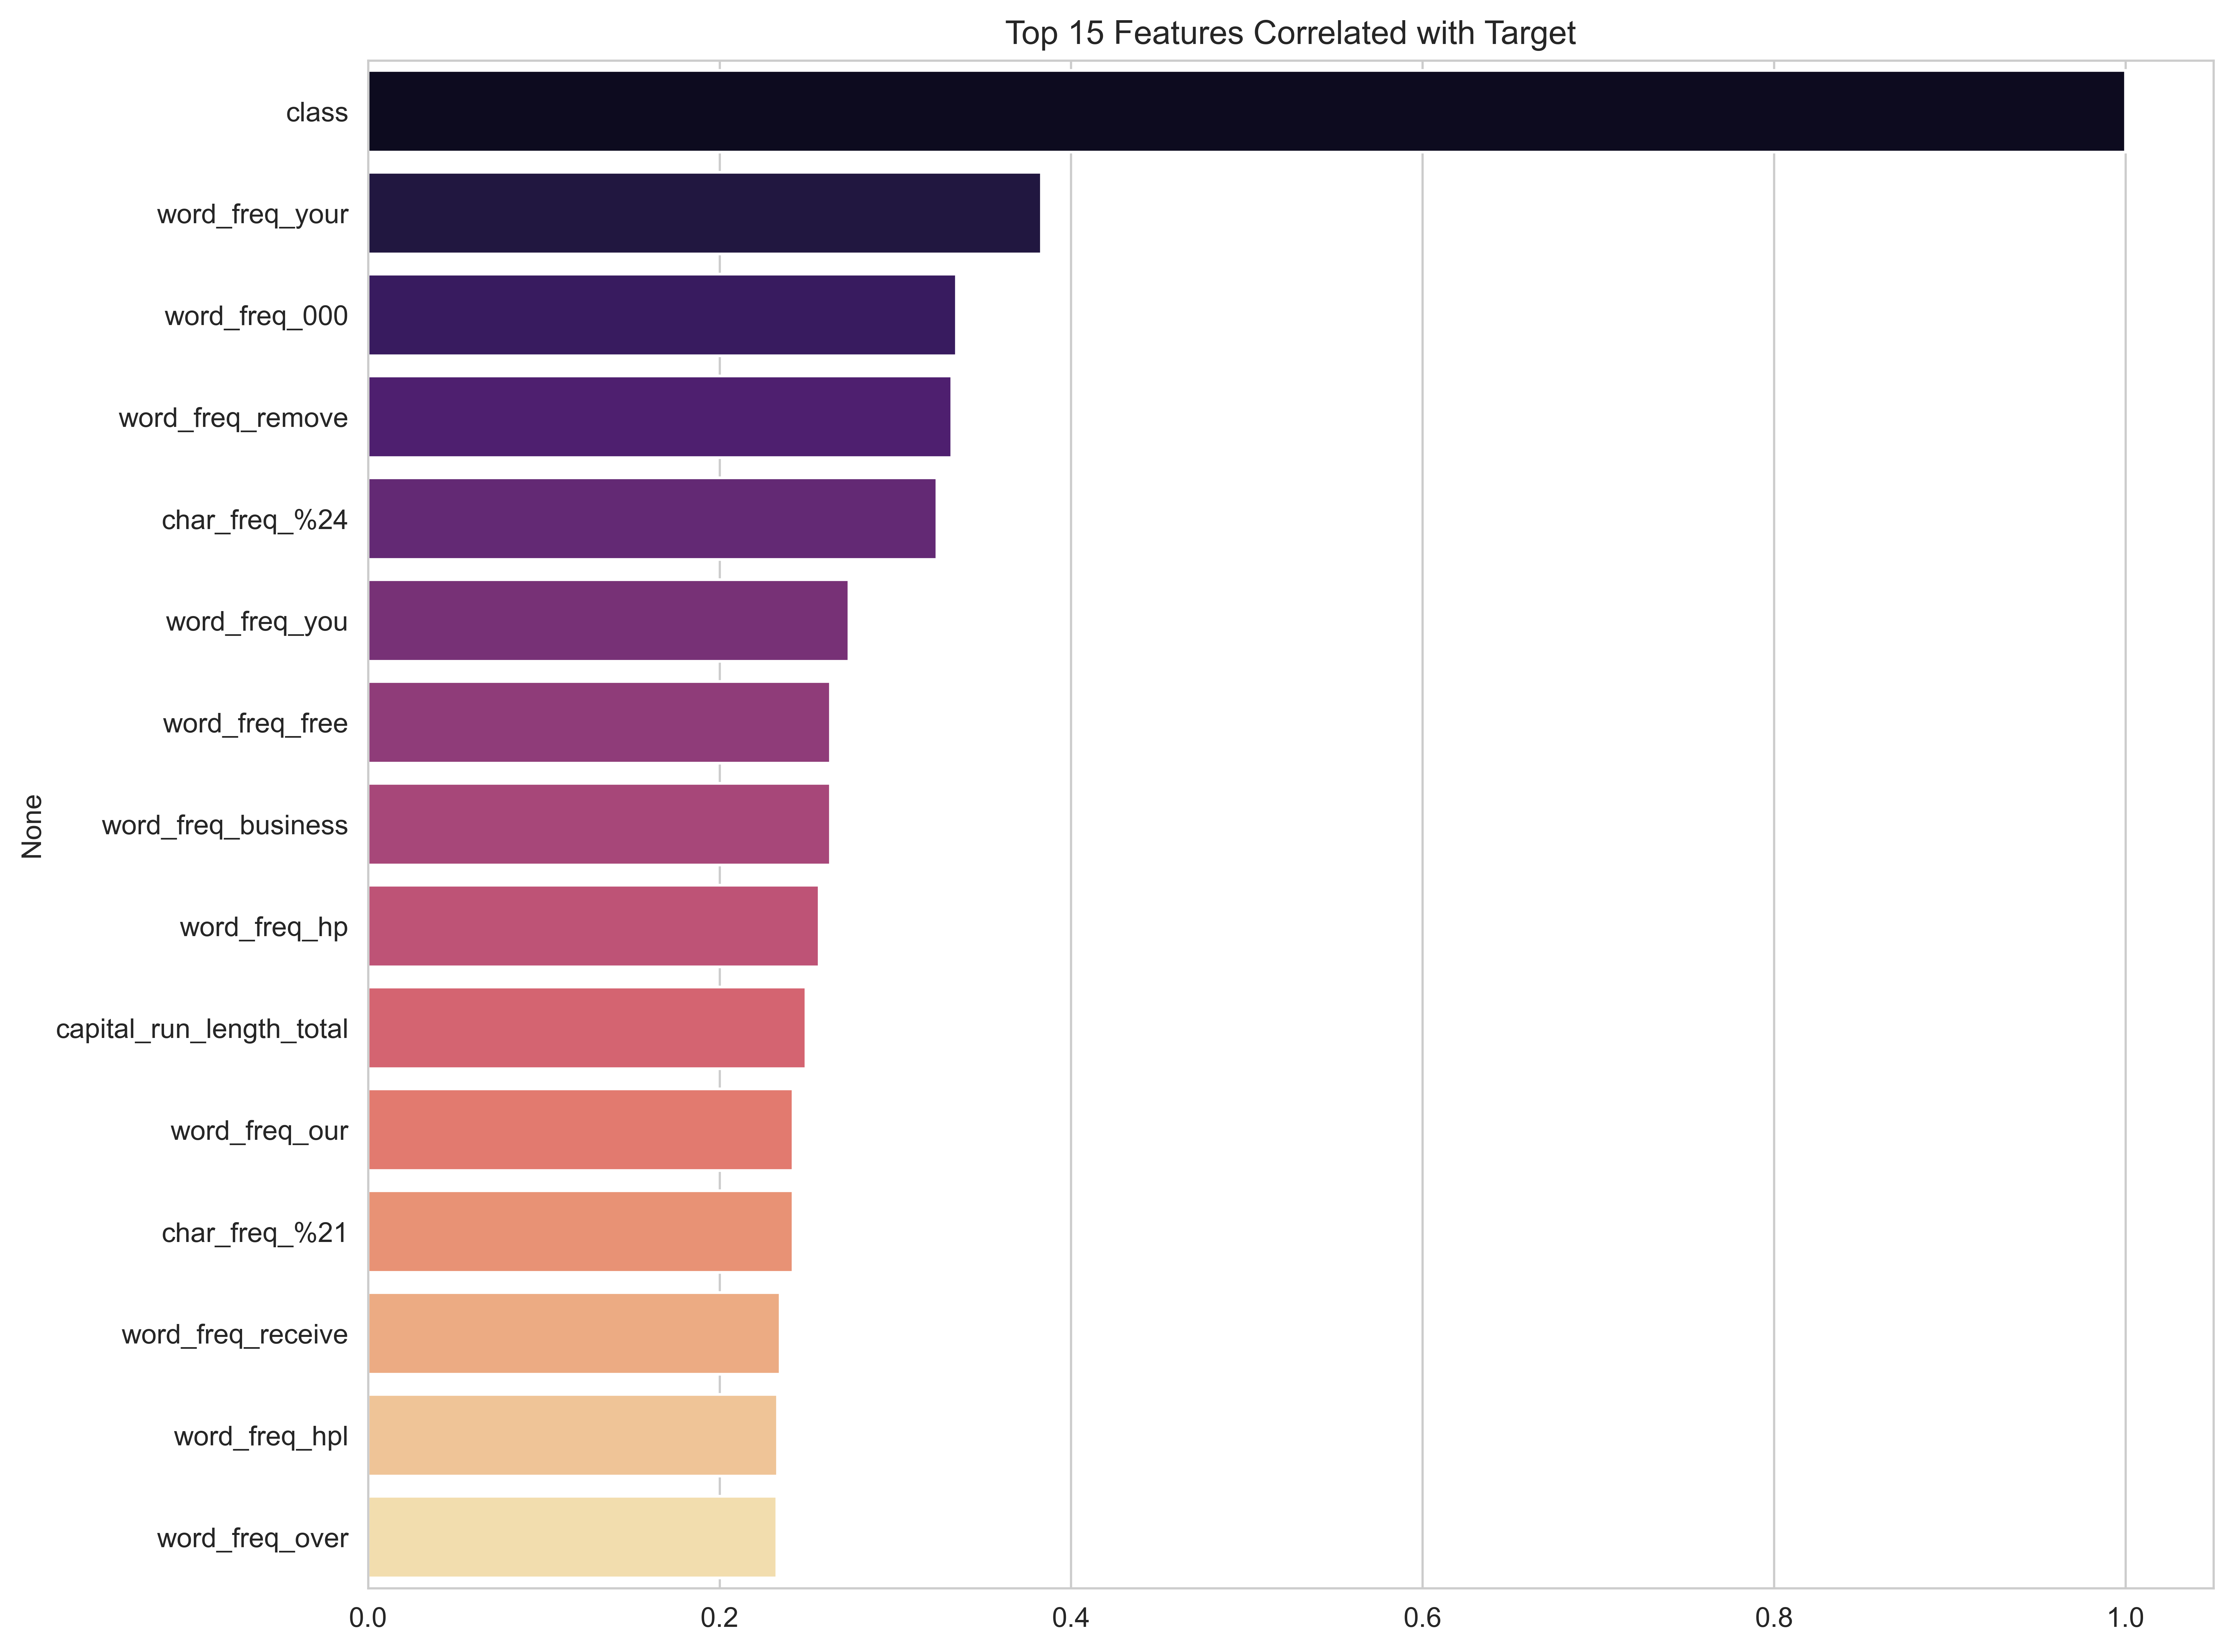
\includegraphics[width=0.8\textwidth]{png/feature_correlation.png}
\caption{Feature Correlation with Target (Top 15)}
\end{figure}

\begin{figure}[h!]
\centering

\includegraphics[width=0.8\textwidth]{png/confusion_matrices.png}
\caption{Confusion Matrices for Logistic Regression and SVM}
\end{figure}

\begin{figure}[h!]
\centering
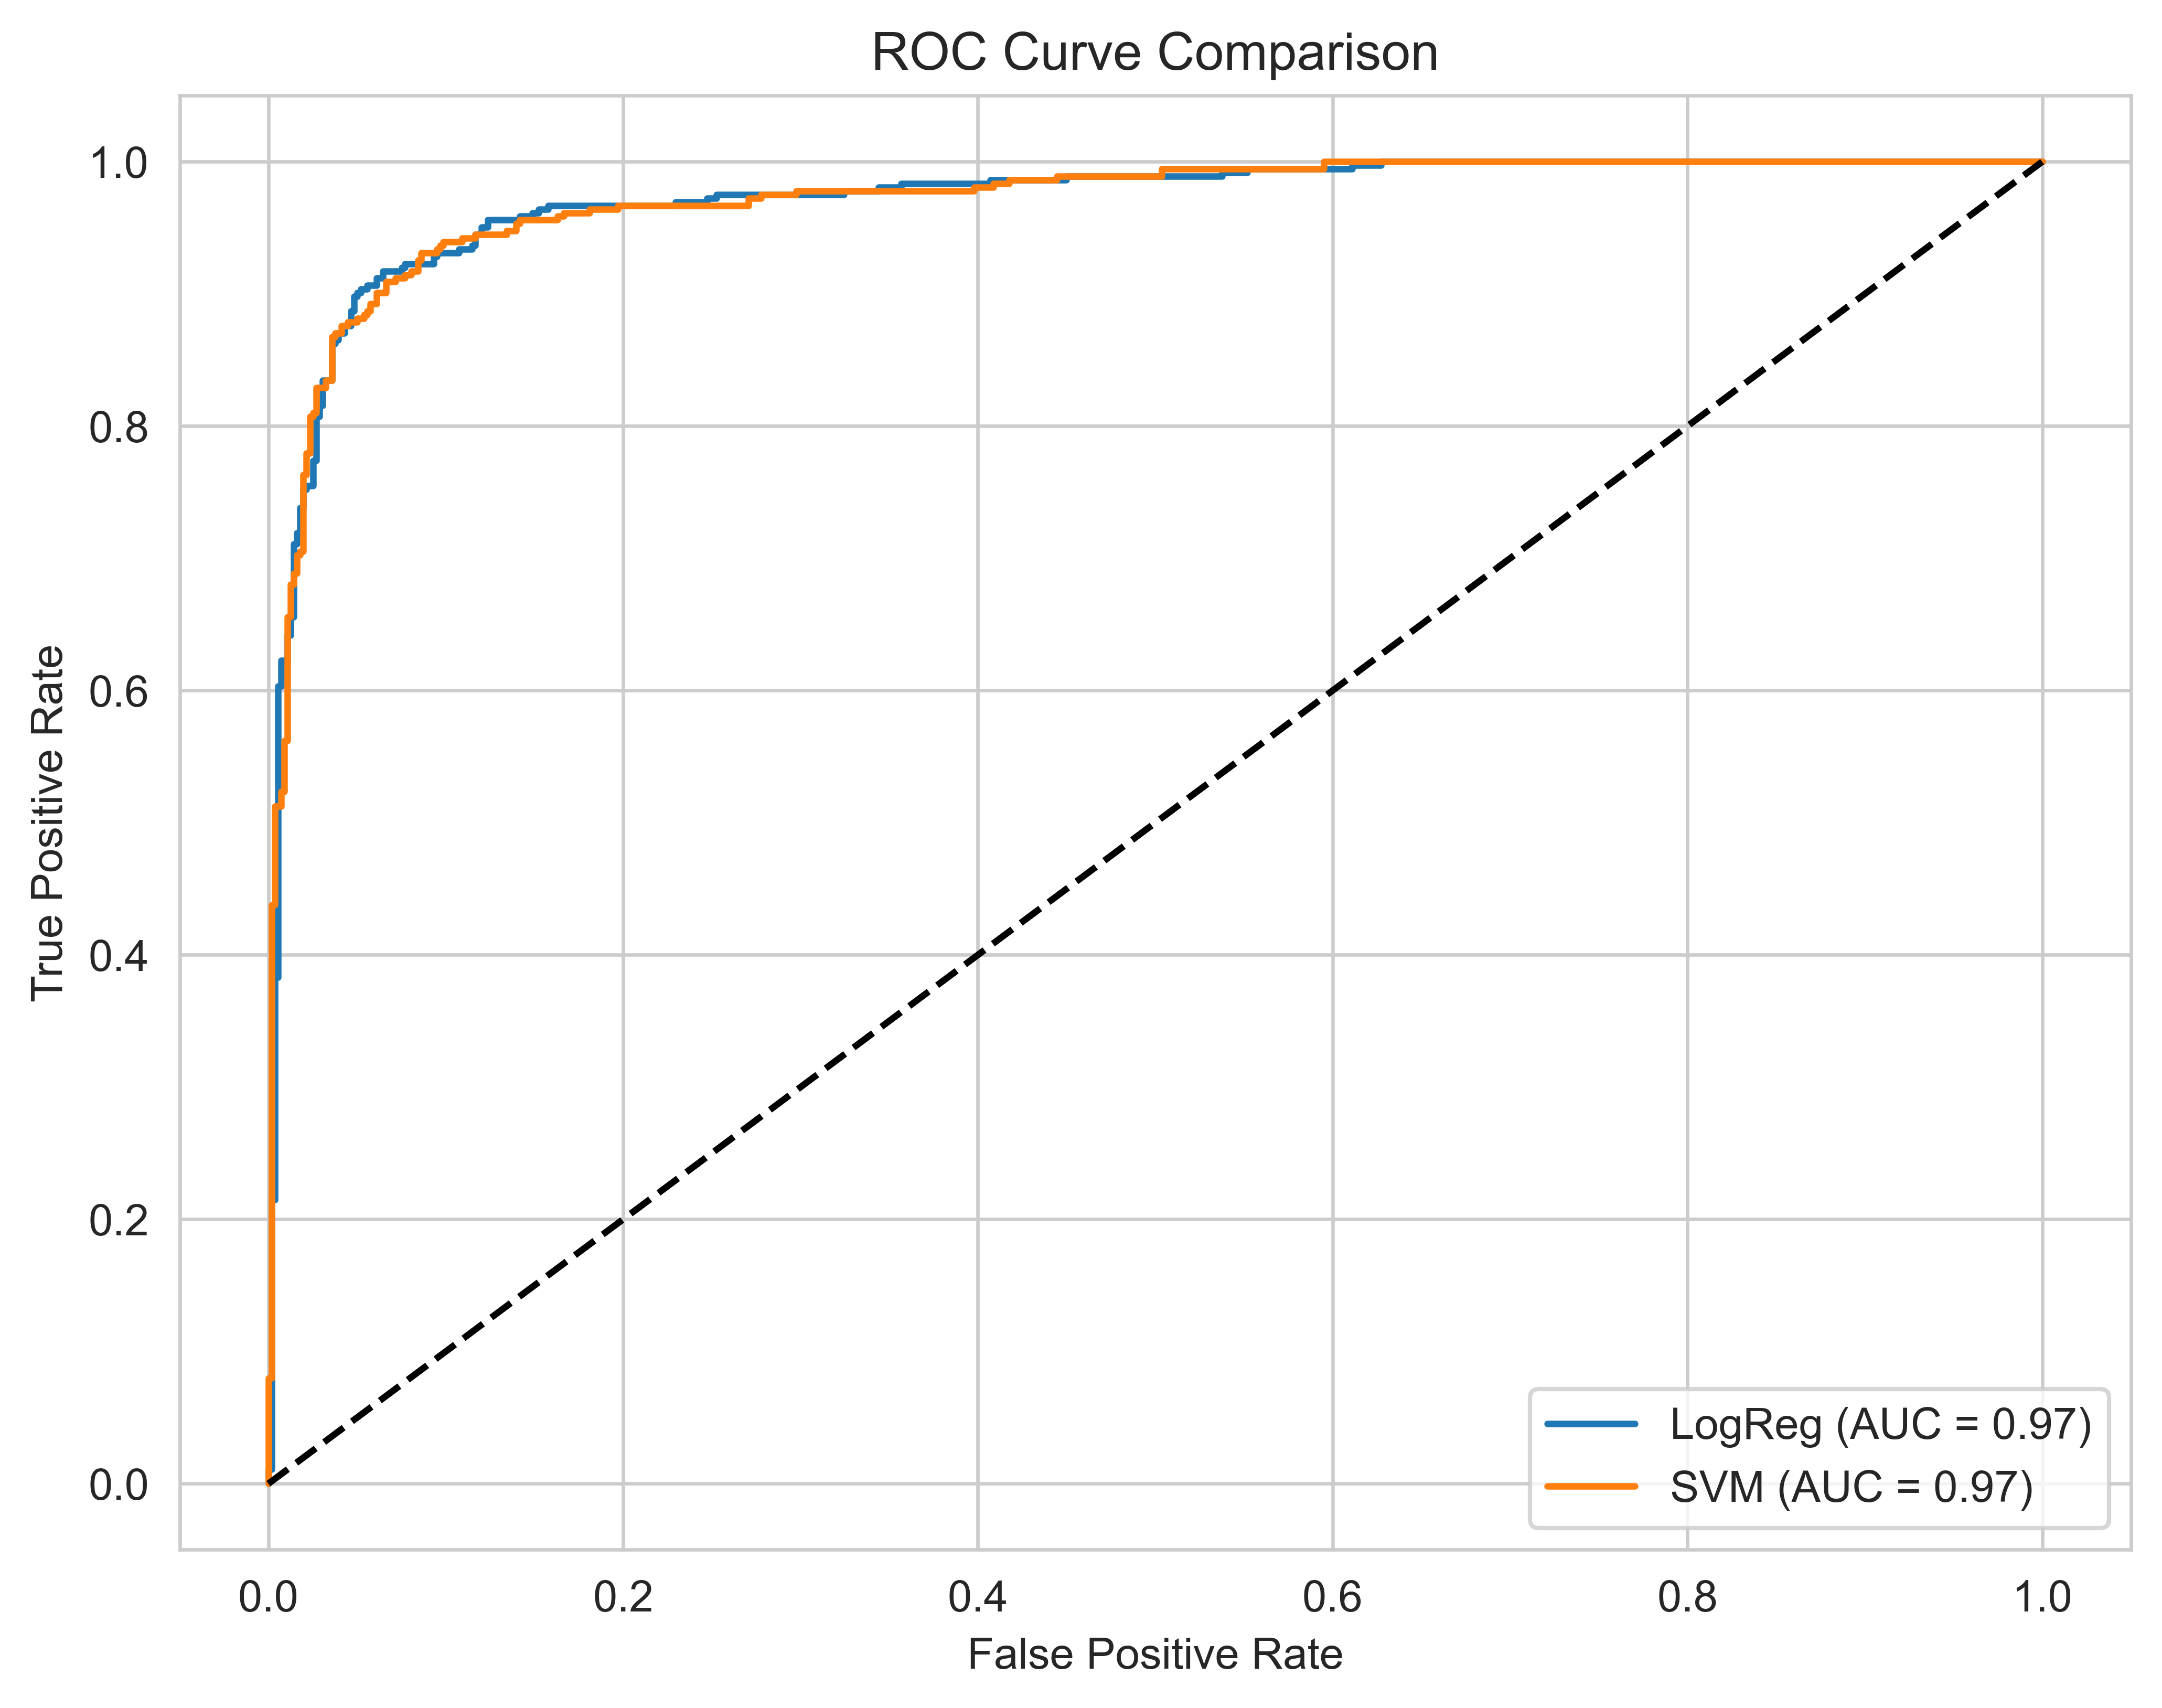
\includegraphics[width=0.6\textwidth]{png/roc_curve.png}
\caption{ROC Curve Comparison between Logistic Regression and SVM}
\end{figure}

\begin{figure}[h!]
\centering
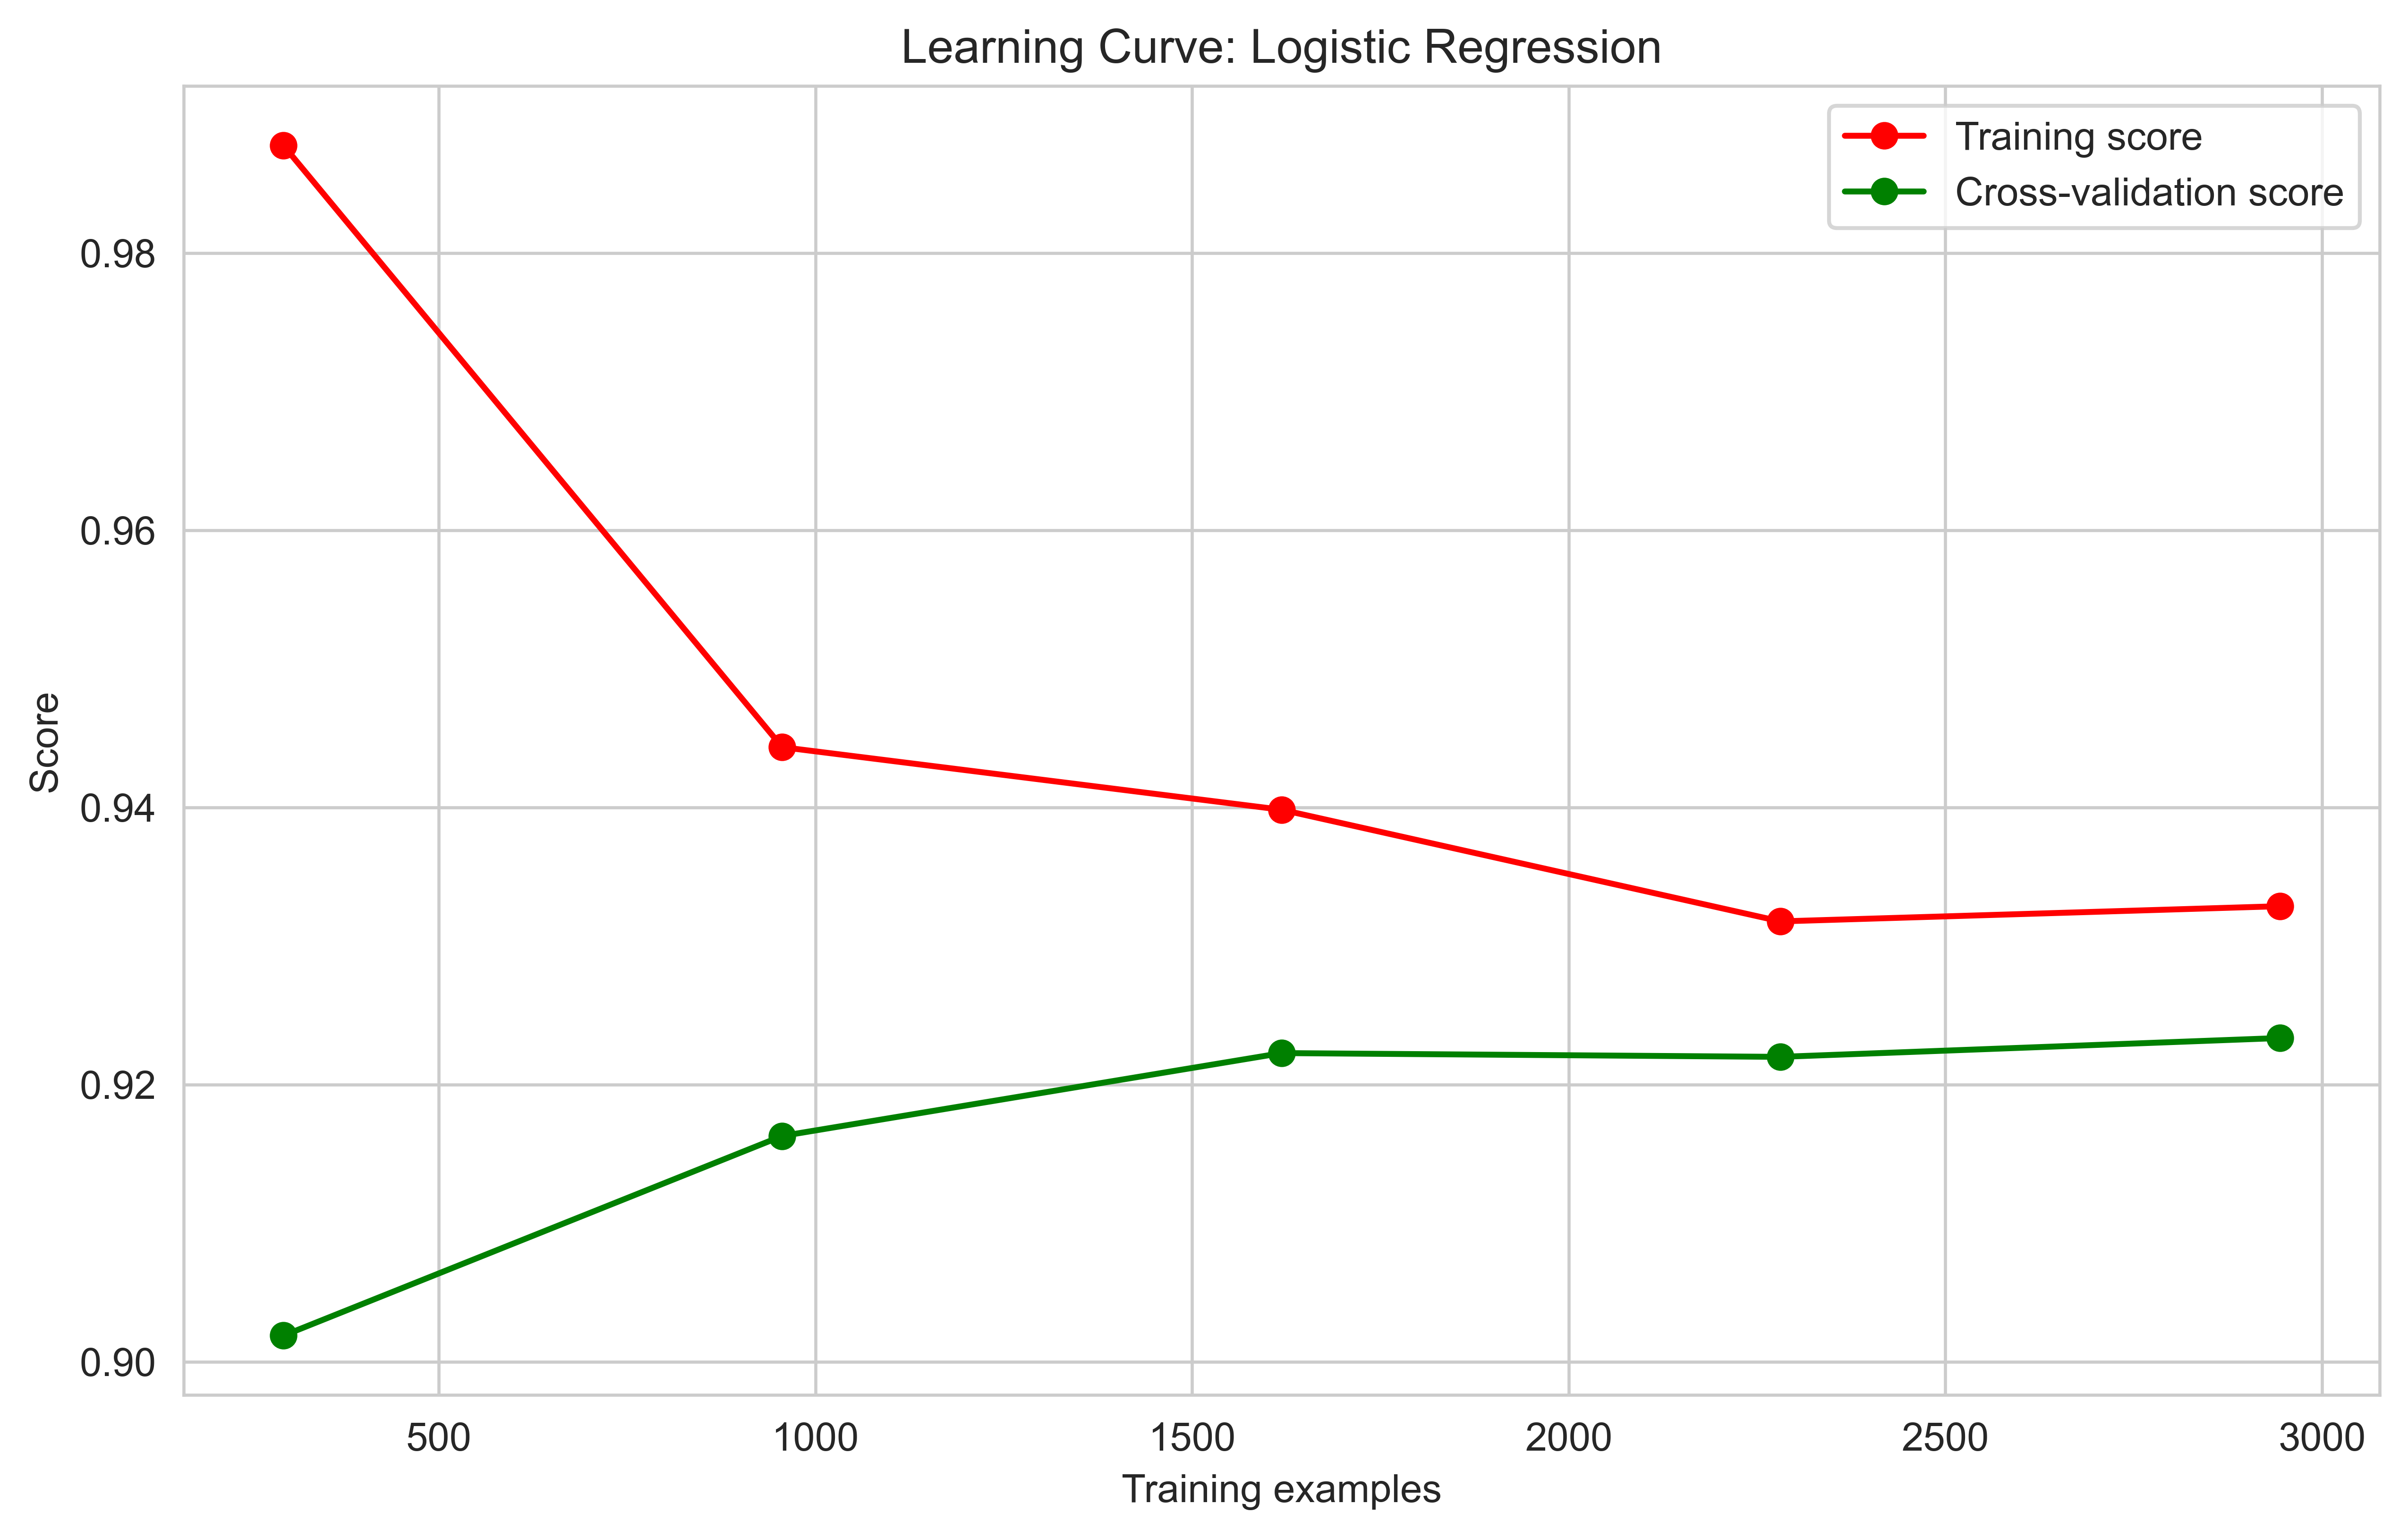
\includegraphics[width=0.8\textwidth]{png/learning_curve_lr.png}
\caption{Learning Curve: Logistic Regression}
\end{figure}

\begin{figure}[h!]
\centering
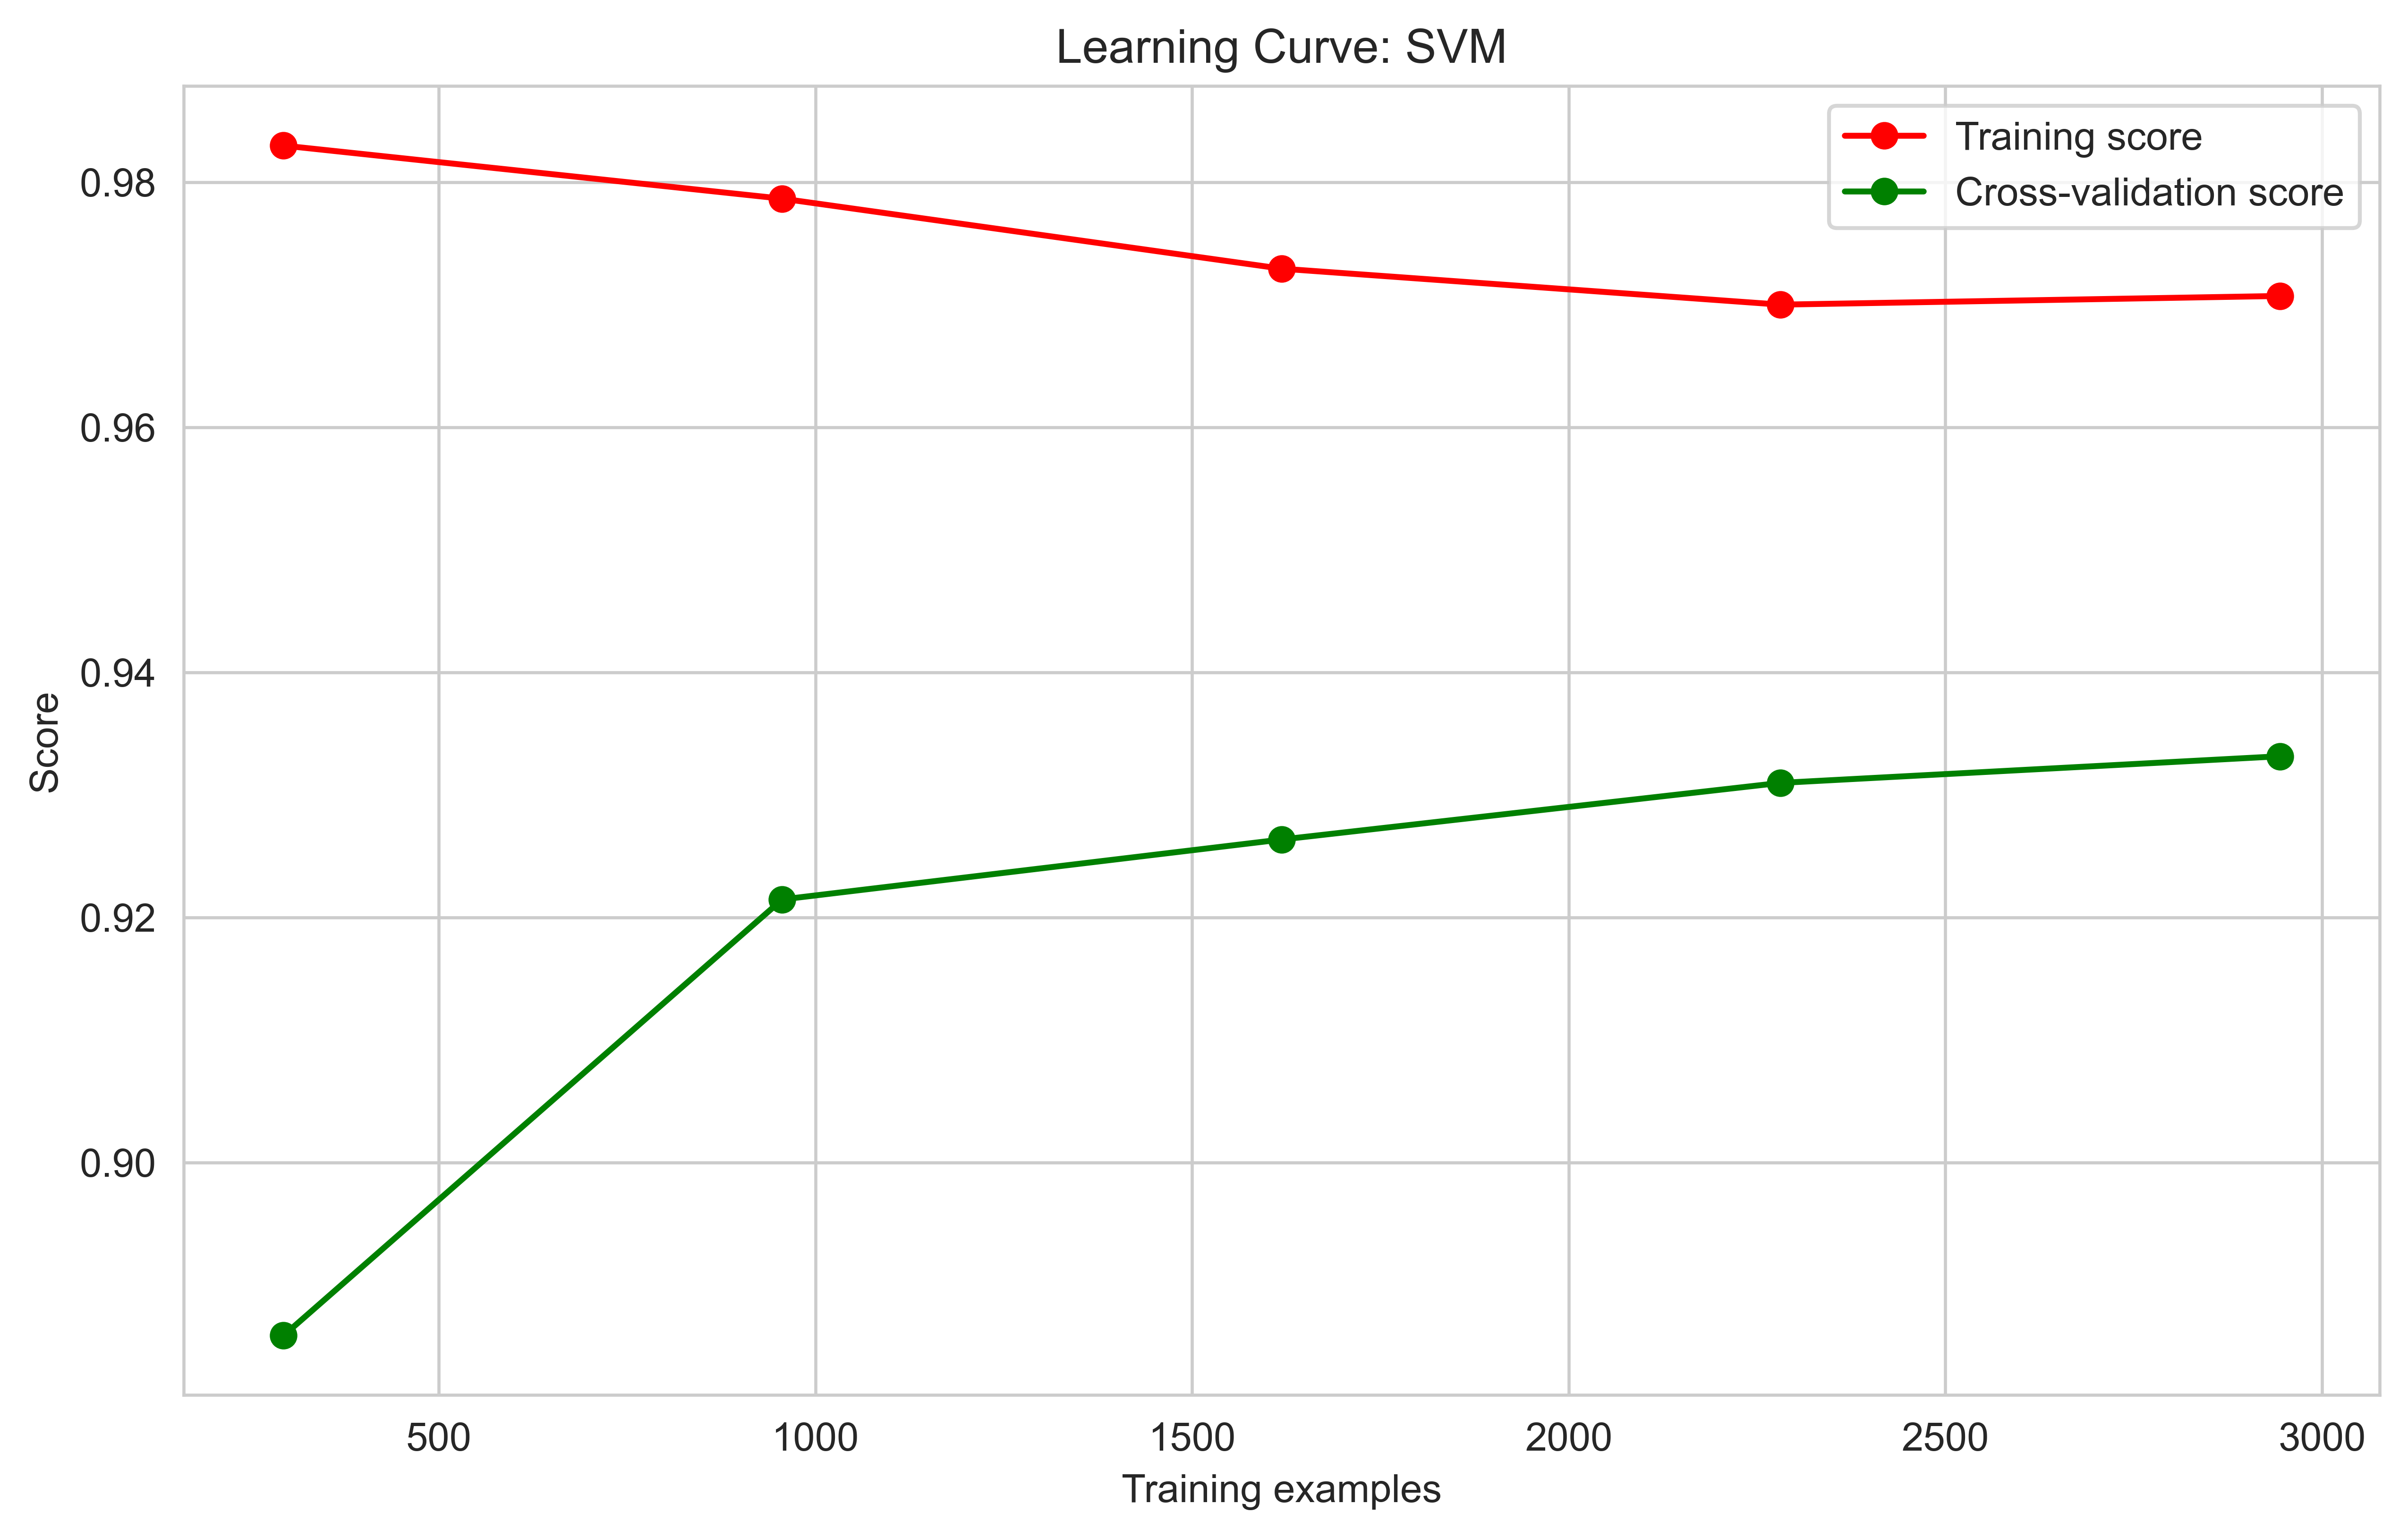
\includegraphics[width=0.8\textwidth]{png/learning_curve_svc.png}
\caption{Learning Curve: SVM (RBF Kernel)}
\end{figure}

%==================================================
\section*{Observations}
\begin{itemize}
\item The best-performing classifier based on cross-validation accuracy is SVM with RBF kernel (93.3\%), though Logistic Regression is highly comparable and significantly faster to train on this dataset.
\item L1 Regularization in Logistic Regression helped in feature selection by shrinking less relevant word and character frequency coefficients to zero, increasing interpretability in the high-dimensional feature space [web:20][web:23].
\item RBF and Linear kernels performed substantially better than Polynomial and Sigmoid, suggesting that the spam data admits a relatively clear but high-dimensional separation boundary that is well captured by linear and RBF decision functions [web:22].
\item Both models show low bias but moderate variance; learning curves indicate that additional training samples could yield marginal gains in generalization, while more advanced ensembles or deep models might further improve performance at the cost of interpretability [web:21][web:24].
\end{itemize}

%==================================================
\section*{Learning Outcomes}
\begin{itemize}
\item Understand probabilistic (Logistic Regression) and margin-based (SVM) classifiers for binary text classification.
\item Apply systematic hyperparameter tuning (Grid Search / Randomized Search) and cross-validation.
\item Evaluate classification models using Accuracy, Precision, Recall, F1 Score, and ROC-AUC, and interpret confusion matrices and learning curves [web:22][web:28].
\item Interpret experimental results to choose an appropriate model based on performance, complexity, and interpretability trade-offs.
\end{itemize}

%==================================================
\section*{References}
\begin{itemize}
\item \href{https://scikit-learn.org/stable/modules/linear_model.html#logistic-regression}{Scikit-learn: Logistic Regression}
\item \href{https://scikit-learn.org/stable/modules/svm.html}{Scikit-learn: Support Vector Machines}
\item \href{https://scikit-learn.org/stable/modules/grid_search.html}{Scikit-learn: Hyperparameter Optimization}
\item \href{https://www.kaggle.com/datasets/somesh24/spambase}{Spambase Dataset – Kaggle}
\item \href{https://archive.ics.uci.edu/ml/datasets/spambase}{UCI ML Repository – Spambase}
\end{itemize}

\end{document}
